\section{Discussion}

\subsection{PCB design}

The use of hierarchical design made the \acrshort{pcb} design process relatively simply. Layout of the Ethernet interface required use of differential signalling, this is the most complex piece of hardware design in this project. Because of tools made specifically for this kind of work in the \acrshort{pcb} layout software, this process is made easier even for inexperienced hardware designers.  

\subsection{PCB production}

It is worth noting that the prototype production run of \acrshort{vcu20}, a sponsor of Revolve NTNU covered all costs of \acrshort{pcb} production. This renders the argument of reducing cost by employing a \acrshort{som} somewhat moot. However, this has not been the case for previous teams, and it is far from certain that it will continue like this in the future.

\subsection{PCB assembly}

Soldering the finished \acrshort{pcb} was done solely by hand without any major problems. The connectors used for the ZX5 module has a \emph{pitch} (distance between the individual pins) of $0.5\si{\milli\metre}$, which is hard to solder by eye. A microscope was used for this part of the soldering, and since Revolve NTNU owns several microscopes this is not regarded as a large issue.   

\subsection{PCB testing}

After finishing assembly, \acrshort{vcu20} underwent a series of tests to ensure correct functioning. During testing, it was discovered that the \acrfull{jtag} interface was incorrectly connected to the ZX5 module. See figure 

\begin{figure}[H]
    \centering
    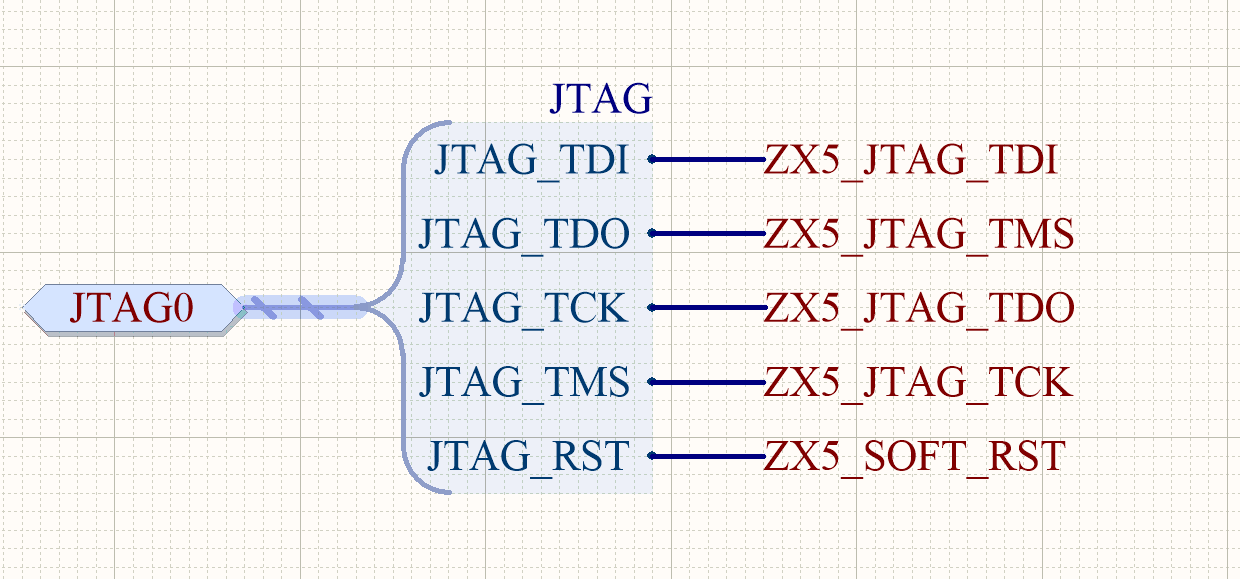
\includegraphics[width=.85\textwidth]{media/jtag_error.png}
    \caption{JTAG interface schematic in Altium Nexus. Notice the signal mismatch as they enter the \emph{harness} (a collection of signals).}
    \label{fig:vcu20_soldered}
\end{figure}

Luckily, this error was recoverable by unsoldering a programming buffer soldering jumper wires to its pads, correcting the error. After performing this fix, the \acrshort{jtag} worked correctly. 


